\chapter{Theoretical Background}\label{chp:theory}

\section{Literature Review}\label{sec:litreview}

The literature review in \Cref{sec:litreview} presents past and present research on utilisation of machine learning method to achieve energy efficient operation. The concept of different modelling approach for ship operation will be discussed in \Cref{sec:ship_modelling}. Generalisation performance of random forest in various research are discussed in \Cref{sec:rf_performance}. Brief summary of the literature review is presented in \Cref{sec:lit_review_conclusion}.\\

\subsection{Modelling Approach for Ship Operation}\label{sec:ship_modelling}

The work by Yan et al. \citep{Yan.2021} provides a thorough review of the different attempts that have been made by different authors to predict different parameters of ship's operation, this includes ship's fuel consumption. Per definition by Haranen et al. \citep{MichaelHaranen.2016}, the modelling of ship operation is categorised into White Box Model (WBM), Black Box Model (BBM) and Grey Box Model (GBM). Machine learning approach is categorised as BBM, BBM approach is defined as purely data driven approach requiring no prior knowledge about the ship operation. The literature review by Yan et al. \citep{Yan.2021} indicated that about $42\%$ of the research utilised BBM model based on machine learning approach.\\ 

Yan et al. \citep{Yan.2021} elaborated further in their work, that BBMs in general have a good fitting ability for unseen data. BBMs based on machine learning model are able to generalise better compared to BBMs based on statistical modelling. With increasing amount of data, better generalisation performance and handling noisy of data should be expected in a BBM model. However, for this same reason, the quality of BBM model is highly dependent on data quantity and quality. BBM model are also generally complex making it challenging to analyse and explain. Shipping industry experts also are having difficulty accepting models that violate the domain knowledge.\\   

From the work of Yan et al. \citep{Yan.2021}, it can be concluded that model accuracy and appropriateness is a significant factor that should be considered when modelling. The model should obey shipping domain knowledge and an intuitive model will help shipping experts analyse its accuracy. For this reason, tree-based model will be considered as it is known for its intuitiveness and interpretability \citep{Breiman.2017}. Breiman et al.\citep{Breiman.2001} even claimed that random forest is the ``most interpretable'' and ``most accurate''. With that,\Cref{sec:rf_performance} will focus on predictive performance of random forest against different machine learning model on different data types and data source. \\

\subsection{Use of AIS Data for Scientific Research}\label{sec:ais_use}

Apart from its intended use as collision avoidance system AIS data have seen potential usage in the field of scientific research. In the third Green House Gas (GHG) study by Smith et al.\citep{T.W.P.Smith.2015}, uses AIS to estimate global shipping emission inventories. Rakke \citep{Rakke2016} proposed a methodology termed ECAIS to calculate ship emissions based on the fuel consumption from AIS data. Through Holtrop-Mennen approximation and literature approximation, the ship's power propulsion can be determined which is subsequently used to predict specific fuel consumption. Wen et al. \citep{Wen.2017} attempted to minimise the Energy Efficiency Operational Indicator (EEOI) using green routing. Recent research by Kim et al. \citep{Kim.2020b} used publicly accessible AIS data, ship static data and environmental data to estimate EEOI  without requiring the actual FOC. The study used big data technology as public data are of large capacity. Generally, the study using AIS data is done to achieve independence from the need to use commercial database. The detail of AIS data will be discussed in \Cref{sec:ais_theo}\\  

\subsection{Prediction Performance of Random Forest}\label{sec:rf_performance}

Majority of the BBM approach based on ML is dominated by ANN \citep{Yan.2021}. However, there are literatures that considered decision tree-based modelling approach to predict fuel consumption. Some example of decision tree based modelling include Decision Tree (DT), Random Forest (RF) and Extra Tree (ET). Soner et al. \citep{Soner.2018} implemented tree-based model, which include bagging, random forest (RF), and bootstrap. In their work, they used data captured from onboard sensors of a ferry to predict speed through water and fuel consumption per hour. From the test dataset, the random forest model described root mean square error (RMSE) of $0.34$ Knots during its prediction of Speed Through Water (STW). Yan et al. \citep{Yan.2020} used random forest (RF) model to minimise fuel consumption for a voyage of a dry bulk ship. The model use ship operational data and sea and weather data from noon report and EMCWF. The prediction performance report from this literature reported mean absolute percentage error (MAPE) of $7.91\%$.\\      

The research by Gkerekos et al. \citep{Gkerekos.2019} highlighted the performance of different machine learning models to predict ship's fuel consumption per day using both noon data and automated data logging and monitoring (ADLM) system from a bulk carrier. This research concludes that tree based model displayed good prediction performance on both noon data and sensor based data. Using default parameters, RF model obtained $R^2$ score of $87.55\%$ and $96.26\%$ for noon-data datasets and sensor-based data respectively. It is also noted that it that the data from a 3-month period in ADLM system would be sufficient to create a model with better performance than the model generated by noon data from a collection period of 2.5 year. This literature also concluded that automatic sensor-based data have the potential to increase the model accuracy score, $R^2$, by $5-7\%$ across different machine learning models.\\

Li et al. \citep{Li.2022} performed more extensive research on the effects of data fusions between meteorological data, ship voyage data and AIS data on different machine learning models to predict the ship's FOC. This research highlighted the advantage of fusing meteorological data and ship voyage data. The evaluation on different model performance indicated that RF are among preferable model candidate that could be used in commercial scale due to its good prediction capability and robustness against different datasets. The findings in this research reported that $R^2$ score are above $96\%$ when deployed on the best datasets and achieved $R^2$ score in range between $74\% - 90\%$ over test data. This literature also exhibited the robustness of RF, as it attained the lowest standard deviation at $0.015$ of the $R^2$ score when evaluated against random splits of datasets.\\

Abebe et al. \citep{Abebe.2020} used different approach in their research by predicting the ship's Speed Over Ground (SOG) instead of FOC. In this work, AIS data and noon-report weather data from 14 tracks and 62 ships are used for the SOG prediction. The observation showed that RF model achieved RMSE of $0.25$ knots, while using $489$ seconds for training. Decision tree achieved RMSE of $0.36$ knots, taking up $52$ seconds for training. This shows that RFR outperforms DTR at cost of computational power.\\

\subsection{Conclusion of Literature Review}\label{sec:lit_review_conclusion}

This literature review described the capability of Random Forest Regressor to predict fuel consumptions and ship speed, irrespective of data source and type of data used. Promising results from different performance measures across different literatures indicated the capability random forest model as predictor. As such, this thesis aims to find optimisation possibilities to extract maximum prediction performance from random forest. Due to the nonlinear, third order function estimate of fuel consumption \citep{Ronen.1982,Ronen.2011}. Accurate prediction of ship speed is paramount to ensure optimal ship operation resulting in increase of profitability. 

\section{Tree-based model}\label{sec:tree_intro}

Random forest belongs to the family of tree-based model and its functional principle stems from decision tree. Decision tree is a non-parametric model that can perform both classification and regression tasks for discrete variable and continuous variable. It is a powerful algorithm, capable of fitting complex datasets. Tree-based model requires very little to no data pre-processing \citep{Geron.2019,Hastie.2009}. To grasp the concept of random forest, The principle working of decision tree will be introduced in depth in \Cref{sec:dt_theo}. It is then followed by \Cref{sec:rf_theo} which presents the principle function behind random forest. Brief explanation for Extra-Trees, method introduced to further improvise random forest, will be presented in \Cref{sec:et_theo}.\\

\subsection{Decision Tree}\label{sec:dt_theo}

Decision tree is a white box model\footnote{This is not to be interchanged with the definition described by Haranen et al. \citep{MichaelHaranen.2016} regarding modelling of ship operation.} \citep{Geron.2019}. In machine learning sense, this means that the model is intuitive, and the structure of the model is interpretable. Thus, the structure of the model can be analysed in detail. To train Decision Trees, \scikit/ \citep{FabianPedregosa.2011} uses the \emph{Classification and Regression Tree} (CART) algorithm \citep{Breiman.2017}. Partition space shown by \Cref{fig:partitionspace} are used to illustrate the decision of CART algorithm. This process can be alternatively represented by the binary tree of \Cref{fig:partitiontree}, observation that satisfies the condition are assigned to the left branch and the opposite is assigned to the right branch. The binary tree representation can be especially helpful when multiple input variables are involved, as the responses can be represented by a single tree \citep{Hastie.2009}.\\

\begin{figure}[h]
\centering
\begin{minipage}[b]{.5\textwidth}
    \centering
    \begin{tikzpicture}[x=0.75pt,y=0.75pt,yscale=-1,xscale=1]
    %uncomment if require: \path (0,433); %set diagram left start at 0, and has height of 433
    
    %Shape: Square [id:dp5731268858272198] 
    \draw   (180,110) -- (370,110) -- (370,300) -- (180,300) -- cycle ;
    %Straight Lines [id:da615072570759449] 
    \draw    (250,110) -- (250,300) ;
    %Straight Lines [id:da8002566967918264] 
    \draw    (300,110) -- (300,300) ;
    %Straight Lines [id:da4409034763483005] 
    \draw    (180,230) -- (250,230) ;
    %Straight Lines [id:da07514682530914596] 
    \draw    (300,170) -- (370,170) ;
    
    % Text Node
    \draw (131,192.4) node [anchor=north west][inner sep=0.75pt]    {$X_{2}$};
    % Text Node
    \draw (261,340.4) node [anchor=north west][inner sep=0.75pt]    {$X_{1}$};
    % Text Node
    \draw (157,222.4) node [anchor=north west][inner sep=0.75pt]    {$t_{2}$};
    % Text Node
    \draw (201,252.4) node [anchor=north west][inner sep=0.75pt]    {$R_{1}$};
    % Text Node
    \draw (201,162.4) node [anchor=north west][inner sep=0.75pt]    {$R_{2}$};
    % Text Node
    \draw (268,192.4) node [anchor=north west][inner sep=0.75pt]    {$R_{3}$};
    % Text Node
    \draw (321,132.4) node [anchor=north west][inner sep=0.75pt]    {$R_{4}$};
    % Text Node
    \draw (321,220.4) node [anchor=north west][inner sep=0.75pt]    {$R_{5}$};
    % Text Node
    \draw (241,310.4) node [anchor=north west][inner sep=0.75pt]    {$t_{1}$};
    % Text Node
    \draw (291,312.4) node [anchor=north west][inner sep=0.75pt]    {$t_{3}$};
    % Text Node
    \draw (381,162.4) node [anchor=north west][inner sep=0.75pt]    {$t_{4}$};
    
    \end{tikzpicture}
    
    \captionof{figure}{Example of partition space \citep{Hastie.2009}} 
    \label{fig:partitionspace}
\end{minipage}%
\begin{minipage}[b]{.5\textwidth}
    \centering
    \begin{tikzpicture}
        \tikzset{level distance=65pt,sibling distance=10pt,edge from parent/.style=
        {draw,edge from parent path={(\tikzparentnode.south)
                                -- +(0,-8pt)
                                -| (\tikzchildnode)}}}
    \Tree [.$X_1\leq t_1$ [.$X_2\leq t_2$ [.$R_1$ ] [.$R_2$ ] ]
        [.$X_1\leq t_3$ [.$R_3$ ]
        [.$X_2\leq t_4$ [.$R_4$ ] [.$R_5$ ] ] ] ]
    \end{tikzpicture}
    \captionof{figure}{Example of partition tree \citep{Hastie.2009}} 
    \label{fig:partitiontree}
\end{minipage}
\end{figure}

Now, we need to understand the principle of selection for the feature $k_t$ and threshold $t_k$. We shall first start with the principle of selection of the threshold $t_k$; Assuming a case with single feature $k$ and response $y$, with $m$ data points. The algorithm starts by looking for possible thresholds. This is determined by calculating the splitting value.\footnote{For example, suppose there are data points at $k = [0.2,0.4]$, then the splitting value is the value in between, i.e., $t_k = 0.3$}. Then, the mean of the response $y$ of partition space $S_1$ and $S_2$ is calculated as seen in \Cref{fig:geron6_5}.\\ 

This step is then followed by calculating the sum of squared error (SSE) of each data points in partition space $S_1$ and $S_2$ and dividing it by the number of data points $m_{s_1}$ and $m_{s_2}$ respectively to obtain the MSE. Subsequently, the MSE from the respective partition space $S_1$ and $S_2$ is summed. The process is then recursively repeated until a threshold $t_k$ that produce minimum sum of MSE is determined. This algorithm is defined by the following cost function $J(k,t_k)$, with $\hat{y}_{S_i}$, being the mean of the response, $y_{S_i}$, in partition space $S_i$. \citep{Geron.2019,Kuhn.2013}:

% \begin{equation}\label{costfun}
%     J(k,t_k) = \frac{m_{\text{left}}}{m}\text{SSE}_\text{S1} + \frac{m_{\text{right}}}{m}\text{SSE}_\text{S2}
%     \begin{cases}
%         \text{SSE}_{S_{i=(1,2)}} = \sum\limits_{i \in \text{node}}(\hat{y}_\text{node} - y^{(i)} )^2 \\
%         \hat{y}_{\text{node}} = \frac{1}{m_{\text{node}}}\sum\limits_{i\in \text{node}} y ^ {(i)}
%     \end{cases}   
% \end{equation}
\begin{equation}\label{eqn:sse}
    \text{MSE}_{S_i} = \frac{1}{m_{S_i}}\text{SSE}_{S_i} \quad \textbf{where} \quad i = (1,2)   
\end{equation}
\begin{equation}\label{eqn:costfun}
    J(k,t_k) = \frac{1}{m_{S_1}}\text{SSE}_{S_1} + \frac{1}{m_{S_2}}\text{SSE}_{S_2}
    \begin{cases}
        \text{SSE}_{S_i} = \sum\limits_{i \in S_i}(\hat{y}_{S_i} - y_{S_i} )^2 \\
        \hat{y}_{S_i} = \frac{1}{m_{S_i}}\sum\limits_{i\in S_i} y
    \end{cases}  
\end{equation}


Once complete, then the partition space is further split into two more regions and this process is recursively continued until a stopping rule is applied. The stopping rule are either when the tree reaches the maximum depth, (This is controlled by the parameter {\tt max\_depth} in \scikit/), or when it cannot find a split that can further reduce MSE. This best split also corresponds to the best possible fit to the predicted value.\\ 

Same principle is also applied when multiple features are present. Consider there are $k_t$ features, then for each respective features $k_1,k_2,\dots,k_t$, The MSE for each of the features is calculated using the cost function $J(k,t_k)$. The feature that can \emph{\textbf{minimise}} the cost function will be selected as the root of the tree. The tree is then grown further by recursively repeating this process \citep{Hastie.2009,Geron.2019}.\\

\begin{figure}[h]
    \centering
    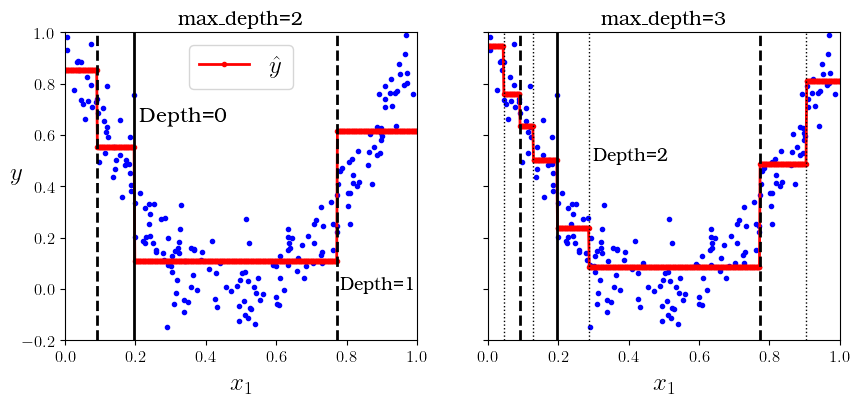
\includegraphics[width=.9\textwidth]{02_figures/fig6_5_partspace_geron09.png}
    \caption{Prediction of two Decision tree regression models \citep{Geron.2019}}
    \label{fig:geron6_5}
\end{figure}

While powerful, decision tree suffers from overfitting when the model is unconstrained. Decision tree makes very few assumptions regarding the training data. Therefore, it will adapt to the training data and fitting it very closely \citep{Geron.2019}. Additionally, an individual tree tends to be unstable, when the data is altered, a completely different set of splits might be found\citep{Hastie.2009,Kuhn.2013}. Therefore, it is necessary to regularise i.e., restrict the decision tree's freedom during the training. Overfitting could be reduced by controlling how deep the tree can grow through the {\tt max\_depth} parameter. Additionally, setting the amount of minimum number of samples a leaf node has, through {\tt min\_samples\_leaf} can alleviate overfitting as well, as shown in \Cref{fig:geron6_6}. However, to address the fundamental drawbacks of decision tree, we shall look into random forest.
\begin{figure}
    \centering
        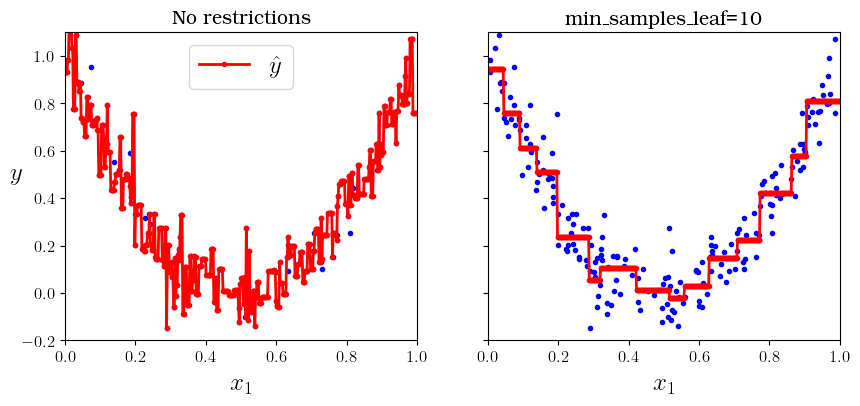
\includegraphics[width=.9\textwidth]{02_figures/fig6_6_paramdepth_geron09.png}
        \caption{Regularising a Decision Tree regressor \citep{Geron.2019}}
        \label{fig:geron6_6}
\end{figure}

\subsubsection{Random Forest}\label{sec:rf_theo}

To understand random forest, the concept of ensemble method shall first be understood. Ensemble is defined as group of predictors such as classifier or regressor. Predictions are aggregated across multiple predictors, for regression task, the prediction is the average across the predictors. This principle is applied to random forest, a group of decision trees is trained on different random set of training data. For regression task, this means the prediction value is the average of the prediction across the decision trees. Such ensemble of decision trees is called \emph{\textbf{Random Forest}} \citep{Hastie.2009,Breiman.2001,TinKamHo.1995}.\\

Ensemble methods achieve the best performance when the predictors are as independent to one another. In statistical sense, this can be achieved by reducing correlation among the trees. This can be realised by adding randomness during tree construction process. For this purpose, random forest utilises \emph{bagging} \citep{Breiman.1996} method (short for \emph{bootstrap aggregating}) during the training process. First, bootstrap sample is created, this means that a sample of the dataset is randomly selected and allowed to appear more than once. This sampling technique is referred to as sampling \emph{with} replacement. Once predictors are trained, then the prediction of the new instance is \emph{aggregated} across the predictors. \citep{Kuhn.2013,Hastie.2009,Geron.2019}\\

To add further randomness, random forest involves random selection of input features $k$ that are considered to split the tree. This means that the feature $k$ that will be used to split the tree is selected from this random subset of feature. The selection for the best feature to be used as the root of the tree and its subsequent node, as well as the stopping rule for the tree's growth is similar to that of decision tree. \citep{Kuhn.2013,Hastie.2009,Geron.2019}\\

These measures introduced in random forest address the tendency of decision tree to overfit. In fact, the instability of decision tree mentioned in \Cref{sec:dt_theo} is exploited in random forest to gain randomness during construction of the tree. Experience from Hastie et al. \citep{Hastie.2009} shown that random forest requires minimal parameter tuning to achieve satisfactory performance while Kuhn et al. \citep{Kuhn.2013} reported that tuning parameter does not have a drastic effect on performance. \\

However, what random forest gains in predictive performance, loses in interpretability. Random forest is considered as Black Box Model (BBM) \citep{Geron.2019}. \footnote{Again, not to be interchanged with the definition described by Haranen et al. \citep{MichaelHaranen.2016} regarding modelling of ship operation.} The randomness means that it is challenging to analyse and describe the decisions made during the selection of the samples and during the selection of the input features. Nevertheless, the interpretability of a single tree in a random forest still holds. As it is still possible to traverse through the tree to reach the predicted value.\\ 

\subsection{Extra-Trees (Extremely Randomised Trees)}\label{sec:et_theo}

Additionally, extra-trees (Extremely Randomised Trees) is introduced by Geurts et al. \citep{Geurts.2006} to further randomise random forest. The key difference lies on how each split is selected; in extra-trees each tree split is selected in random instead of searching for the best split. This technique saves computational power, as searching for best split is one of the tasks that takes up most computational power \citep{Geron.2019}. Extra-trees also do not bootstrap the samples, which mean it samples \emph{without} replacement.\\

% Overview of the tree-based model discussed in \Cref{dt_theo} and \Cref{rf_theo} can be summarised in \Cref{table_trees}:

% \begin{table}[ht]
%     % \small
%     \centering
%     \resizebox {\textwidth}{!}
%     {\begin{tabular}{ |p{5cm}|p{3cm}|p{3cm}|p{3cm}|  }
%     \hline
%     \multicolumn{1}{|c|}{\textbf{Model}} & \multicolumn{1}{|c|}{\textbf{Decision Tree}}  & \multicolumn{1}{|c|} {\textbf{Random Forest}} & \multicolumn{1}{|c|}{\textbf{Extra-Trees}}\\
%     \hline
%     Number of trees & \multicolumn{1}{|c|}{1} & \multicolumn{1}{|c|}{Many} & \multicolumn{1}{|c|}{Many}\\
%     \hline
%     Features considered for split at each node &   \multicolumn{1}{|c|}{All features}  & \multicolumn{1}{|c|}{Random subset of features} & \multicolumn{1}{|c|}{Random subset of features} \\
%     \hline
%     Bootstrapping & \multicolumn{1}{|c|}{Not applied} & \multicolumn{1}{|c|}{Yes} & \multicolumn{1}{|c|}{No}\\
%     \hline
%     Split Rule  & \multicolumn{1}{|c|}{Best split} & \multicolumn{1}{|c|}{Best split}& \multicolumn{1}{|c|}{Random split}\\
%     \hline
%     \end{tabular}}
% \caption{Comparison of tree based model}\label{table_trees}
% \end{table}

\section{AIS Data}\label{sec:ais_theo}

Automatic Identification System (AIS) is an automated tracking system onboard ships to automatically transmit information about the ship to other ships and coastal authorities. As part of the revised new chapter V of SOLAS\footnote{International convention for the Safety of Lives at Sea} regulation. In 2000, International Maritime Organization (IMO) requires installation of AIS class A equipment on all ships of 300 gross tonnage and upward engaged on international voyages, cargo ships of 500 gross tonnages and upwards not engaged on international voyages and all passenger ships irrespective of size. This requirement is then made compulsory to all ships by 2004. \citep{Rakke2016,webimo.2014}\\

AIS uses Very High Frequency (VHF) with special protocol for communication system for information exchange between the ships. This information will be received by either ships directly, buoys, land based station and satellites. The information transmitted by AIS is distinguished into three different types. \textbf{Static information} which is entered into the AIS on installation. \textbf{Dynamic information}, which is automatically updated from the ship's sensors connected to AIS and \textbf{voyage-related information}, which might need to be manually entered and updated during the voyage. The structure of the AIS data that is relevant to this thesis is summarised in \Cref{tbl:AIS_struct}\citep{webimo.2014}.\\

AIS is also further differentiated by its equipment class. The classification is based on the reporting interval and the type of information that is conveyed. \textbf{Class A} autonomously report their position within 2-10 seconds interval, depending on the state of ship's movement. The reporting interval is less frequent at 3 minutes, When the ship is at anchor or moored and moving slower than 3 knots. Class A AIS is also capable of sending safety related information, meteorological and hydrological data, electronic broadcast to mariners and marine safety messages. \textbf{Class B} reports at longer interval and at a lower power. They can only receive safety related messages, not send them. \citep{Rakke2016,webimo.2014}\\
\begin{table}
    % \small
    % \centering
    % \resizebox {\textwidth}{!}
    {\begin{tabular}{ |p{6cm}|p{9cm}|  }
    \hline
    \textbf{Information Item} & \textbf{Description} \\
    \hline
    \multicolumn{2}{|l|}{\textbf{Static}}\\
    \hline
    MMSI & MMSI number of vessel\\
    \hline
    Callsign & Callsign of vessel \\
    \hline
    Name & Name of the vessel \\
    \hline
    IMO & IMO number of the vessel \\
    \hline
    Length & Length of vessel \\
    \hline
    Width & Width of vessel \\
    \hline
    Ship Type & Describes the AIS ship type of this vessel \\
    \hline
    \multicolumn{2}{|l|}{\textbf{Dynamic}}\\
    \hline
    Ship's position & Automatically updated from position sensor connected to AIS. Longitude and Latitude.\\
    \hline
    Position time stamp in UTC & Automatically updated from ship's main position sensor. Format: DD\slash MM\slash YYYY HH:MM:SS\\
    \hline
    Course over Ground (COG) & \emph{\textbf{If available}}, automatically updated from ship's main position sensor connected to AIS.\\  
    \hline
    Speed Over Ground (SOG) & \emph{\textbf{If available}}, automatically updated from the position sensor connected to AIS.\\
    \hline
    Heading & Automatically updated from the ship's heading sensor connected to AIS\\
    \hline
    Navigational status & Navigational status information has to be manually entered by the Officer on Watch (OOW) and changed as necessary. For example : ``\emph{underway by engines}'',``\emph{engaged in fishing}'',``\emph{at anchor}''.\\
    \hline
    Rate of Turn (ROT) & \emph{\textbf{If available}}, Automatically updated from the ship's ROT sensor or derived from
    the gyro.\\
    \hline
    \multicolumn{2}{|l|}{\textbf{Voyage Related}}\\
    \hline
    Ship's draught & To be manually entered at the start of the voyage using the
    maximum draft for the voyage and amended as required \\
    \hline 
    (Hazardous) Cargo Type & Type of cargo from AIS message.\\
    \hline
    Destination and ETA & To be manually entered at the start of the voyage and kept up to
    date as necessary.\\
    \hline
    \end{tabular}}
\caption{Structure of AIS data \citep{webimo.2014}}\label{tbl:AIS_struct}
\end{table}

\subsection{Current Correction}\label{sec:curr_corr}

As indicated in \Cref{tbl:AIS_struct}, the speed shown in AIS is the speed over ground (SOG). However, for calculation of ship's fuel consumption, the actual speed i.e. speed through water (STW) is required. This can be achieved by correcting the SOG for the current speed, in consideration of the research by Zhou et al. \citep{Zhou.2017} which shows the impact of current on ship's SOG. This correction is performed by considering the current speed $V_c$ and the direction of the current $\gamma$ \emph{with respect to True North}. In principle, STW will be greater than SOG, when the current is moving against the current as the ship tries to compensate for the current to maintain the SOG. Similarly, the STW will be greater than the SOG when the current is moving in the same direction of the ship movement. \\

To calculate the correction, this study will adopt the methodology proposed by Kim et al. \citep{Kim.2020b} and Yang et al. \citep{Yang.2020}. The $x$ and $y$ component of SOG can be obtained through vector decomposition using the ship's heading angle $\alpha$ \emph{with respect to True North}. Similar vector decomposition is also performed for current speed $V_{\text{current}}$, it is resolved with current direction $\gamma$ \emph{with respect to True North}:\\
\begin{equation}\label{eqn:sogx}
    V_{\text{SOG}}^x = V_{\text{SOG}}\cdot\sin(\alpha)   
\end{equation}
\begin{equation}\label{eqn:sogy}
    V_{\text{SOG}}^y = V_{\text{SOG}}\cdot\cos(\alpha)   
\end{equation} 
\begin{equation}\label{eqn:vcurrx}
     V_{\text{current}}^x = V_{\text{current}}\cdot\sin(\gamma)   
\end{equation}
\begin{equation}\label{eqn:vcurry}
    V_{\text{current}}^y = V_{\text{current}}\cdot\cos(\gamma)   
\end{equation}
Then the resulting equation to determine STW, including the current compensation, is given by:\\
\begin{equation}\label{eqn:stwx}
    V_{\text{STW}}^x = V_{\text{SOG}}^x - V_{\text{current}}^x    
\end{equation}
\begin{equation}\label{eqn:stwy}
    V_{\text{STW}}^y = V_{\text{SOG}}^y - V_{\text{current}}^y      
\end{equation}
\begin{equation}\label{eqn:stwabs}
    V_{\text{STW}} = \sqrt{(V_{\text{STW}}^x)^2 + (V_{\text{STW}}^y)^2} 
\end{equation}

\section{Weather data}\label{sec:weather_theo}

\section{Calculation of Fuel Oil Consumption}\label{sec:foc_calc}













% \begin{tikzpicture}[x=0.75pt,y=0.75pt,yscale=-1,xscale=1]
%     %uncomment if require: \path (0,452); %set diagram left start at 0, and has height of 452
    
%     %Shape: Axis 2D [id:dp697661158302031] 
%     \draw  (220,297.8) -- (517.5,297.8)(249.75,80) -- (249.75,322) (510.5,292.8) -- (517.5,297.8) -- (510.5,302.8) (244.75,87) -- (249.75,80) -- (254.75,87)  ;
%     %Image [id:dp23308396965327827] 
%     \draw (245,305) node [rotate=-40.58] {
\includegraphics[width=26.87pt,height=72.39pt]{02_figures/ferry.jpg}};
% \end{tikzpicture}




% \subsection{Ship speed}


% \subsection{Modelling}



% Phased out, but might be useful

% Might be useful for multiple images !
% \begin{figure}[h]
% \centering
% \begin{minipage}[t]{.5\textwidth}
%     \centering
%     % \begin{figure}
%     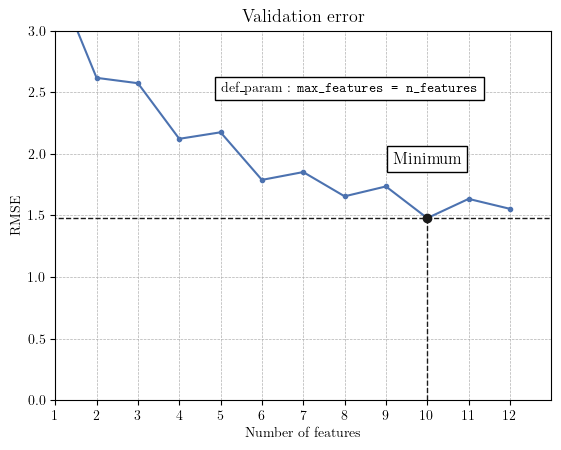
\includegraphics[width=\textwidth]{02_figures/featureserrro.png}
%     % \end{figure}
%     \captionof{figure}{Effects of number of features on RMSE}
%     \label{fig:featureserror}
% \end{minipage}%
% \begin{minipage}[t]{.5\textwidth}
%     \centering
%     % \begin{figure}
%     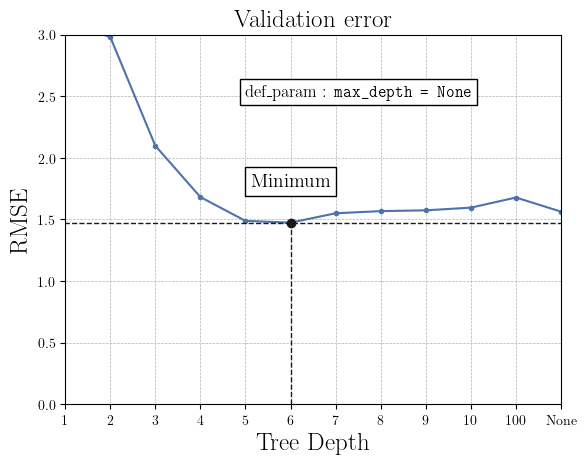
\includegraphics[width=\textwidth]{02_figures/depthError.png}
%     % \end{figure}
%     \captionof{figure}{Effects of tree depth on RMSE}
%     \label{fig:deptherror}
% \end{minipage}
% \end{figure}

% \begin{figure}[h]
%     \centering
%         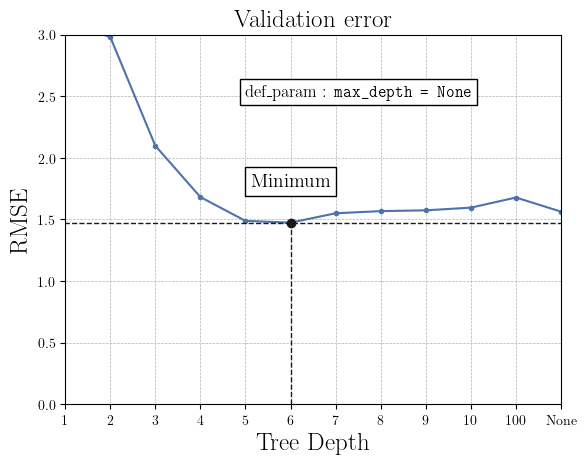
\includegraphics[width=.5\textwidth]{02_figures/depthError.png}
%         \caption{Effect of tree depth on RMSE for validation dataset}
%         \label{fig:Tree Depth Error}
% \end{figure}

% \begin{enumerate}
%     \item Possible thresholds are determined by calculating the splitting value (For example, suppose there are data points at $X = [0.2,0.4]$, then the splitting value is the value in between i.e. $t_k = 0.3$)
%     \item Calculate the mean of data points of the left and right partition space respectively, Defined by the following equation $\hat{y}_{node} = \frac{1}{m_{node}}\sum\limits_{i\in node} y ^ {(i)}$
%     \item Calculate the mean squared error (MSE) of each data points in its respective partition space. Through the equation $MSE_{node} = \sum\limits_{i\in node}(\hat{y}_{node} - y^{(i)} )^2$ 
%     \item The MSE from the respective partition space is summed.
%     \item Step $1 - 4$ is recursively repeated, until the minimum of the cost function $J(X,T_k)$, i.e. minimum MSE, is determined:
%      \begin{equation}\label{costfun}
%         J(X,t_k) = \frac{m_{left}}{m}MSE_{left} + \frac{m_{right}}{m}MSE_{right}
%         \begin{cases}
%             MSE_{node} = \sum\limits_{i\in node}(\hat{y}_{node} - y^{(i)} )^2 \\
%             \hat{y}_{node} = \frac{1}{m_{node}}\sum\limits_{i\in node} y ^ {(i)}
%         \end{cases}   
%     \end{equation}
% \end{enumerate} 